% 2010 年福建卷文科第 20 题：长方体 ABCD-A1B1C1D1 与过 EH 的平面 EFGH。
% 来源 PDF：普通高考/2010/2010福建文.pdf，SHA-256 56e9e7a7fe9733a605b2d88773e59f83f49c173184cc77d721633adf13c16b78。
% 原页：第 2 页（A3 三栏）第 1 栏下部，书页码 592。
% 重绘依据：照原页斜二测画法，前面 ABB1A1 为矩形、后底面按右上方向平移；
%   E 在棱 A1B1 上、H 在棱 D1C1 上且 EH∥A1D1；F 在棱 BB1 上、G 在棱 CC1 上，
%   截面 EFGH 中 EF∥HG、EH∥FG。
%   实线为可见棱与截面的 EH、EF、FG；虚线为被遮挡的棱 AD、DC、DD1 以及位于后表面 DCC1D1 内的截面边 HG。
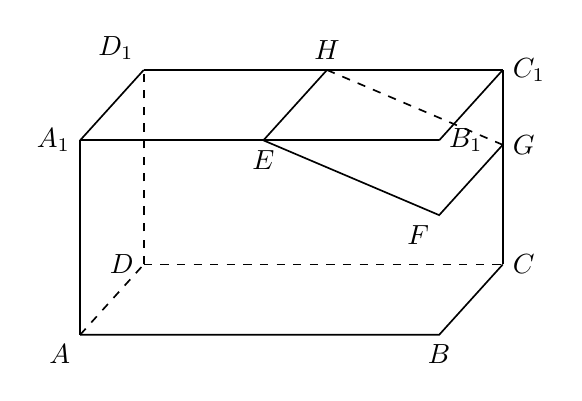
\begin{tikzpicture}[scale=0.95, semithick]
  \coordinate (A)  at (0,0);
  \coordinate (B)  at (4.8,0);
  \coordinate (C)  at (5.65,0.94);
  \coordinate (D)  at (0.85,0.94);
  \coordinate (A1) at (0,2.6);
  \coordinate (B1) at (4.8,2.6);
  \coordinate (C1) at (5.65,3.54);
  \coordinate (D1) at (0.85,3.54);
  \coordinate (E)  at (2.45,2.6);
  \coordinate (H)  at (3.30,3.54);
  \coordinate (F)  at (4.8,1.60);
  \coordinate (G)  at (5.65,2.54);
  % 可见棱
  \draw (A) -- (B) -- (C);
  \draw (C) -- (C1);
  \draw (A) -- (A1);
  \draw (A1) -- (B1);
  \draw (B1) -- (C1);
  \draw (A1) -- (D1);
  \draw (D1) -- (C1);
  % 截面 EFGH（HG 位于后表面内，画虚线）
  \draw (E) -- (F) -- (G);
  \draw (H) -- (E);
  \draw[dashed] (G) -- (H);
  % 被遮挡的棱
  \draw[dashed] (A) -- (D);
  \draw[dashed] (D) -- (C);
  \draw[dashed] (D) -- (D1);
  % 顶点标注
  \node[below left]  at (A)  {$A$};
  \node[below]       at (B)  {$B$};
  \node[right]       at (C)  {$C$};
  \node[left]        at (D)  {$D$};
  \node[left]        at (A1) {$A_1$};
  \node[right]       at (B1) {$B_1$};
  \node[right]       at (C1) {$C_1$};
  \node[above left]  at (D1) {$D_1$};
  \node[below]       at (E)  {$E$};
  \node[above]       at (H)  {$H$};
  \node[below left]  at (F)  {$F$};
  \node[right]       at (G)  {$G$};
\end{tikzpicture}
